 %  LaTeX support: latex@mdpi.com 
%  For support, please attach all files needed for compiling as well as the log file, and specify your operating system, LaTeX version, and LaTeX editor.

%=================================================================
\documentclass[mathematics,article,submit,pdftex,moreauthors]{Definitions/mdpi} 

%--------------------
% Class Options:
%--------------------
%----------
% journal
%----------
% Choose between the following MDPI journals:
% acoustics, actuators, addictions, admsci, adolescents, aerobiology, aerospace, agriculture, agriengineering, agrochemicals, agronomy, ai, air, algorithms, allergies, alloys, analytica, analytics, anatomia, animals, antibiotics, antibodies, antioxidants, applbiosci, appliedchem, appliedmath, applmech, applmicrobiol, applnano, applsci, aquacj, architecture, arm, arthropoda, arts, asc, asi, astronomy, atmosphere, atoms, audiolres, automation, axioms, bacteria, batteries, bdcc, behavsci, beverages, biochem, bioengineering, biologics, biology, biomass, biomechanics, biomed, biomedicines, biomedinformatics, biomimetics, biomolecules, biophysica, biosensors, biotech, birds, bloods, blsf, brainsci, breath, buildings, businesses, cancers, carbon, cardiogenetics, catalysts, cells, ceramics, challenges, chemengineering, chemistry, chemosensors, chemproc, children, chips, cimb, civileng, cleantechnol, climate, clinpract, clockssleep, cmd, coasts, coatings, colloids, colorants, commodities, compounds, computation, computers, condensedmatter, conservation, constrmater, cosmetics, covid, crops, cryptography, crystals, csmf, ctn, curroncol, cyber, dairy, data, ddc, dentistry, dermato, dermatopathology, designs, devices, diabetology, diagnostics, dietetics, digital, disabilities, diseases, diversity, dna, drones, dynamics, earth, ebj, ecologies, econometrics, economies, education, ejihpe, electricity, electrochem, electronicmat, electronics, encyclopedia, endocrines, energies, eng, engproc, entomology, entropy, environments, environsciproc, epidemiologia, epigenomes, est, fermentation, fibers, fintech, fire, fishes, fluids, foods, forecasting, forensicsci, forests, foundations, fractalfract, fuels, future, futureinternet, futurepharmacol, futurephys, futuretransp, galaxies, games, gases, gastroent, gastrointestdisord, gels, genealogy, genes, geographies, geohazards, geomatics, geosciences, geotechnics, geriatrics, grasses, gucdd, hazardousmatters, healthcare, hearts, hemato, hematolrep, heritage, higheredu, highthroughput, histories, horticulturae, hospitals, humanities, humans, hydrobiology, hydrogen, hydrology, hygiene, idr, ijerph, ijfs, ijgi, ijms, ijns, ijpb, ijtm, ijtpp, ime, immuno, informatics, information, infrastructures, inorganics, insects, instruments, inventions, iot, j, jal, jcdd, jcm, jcp, jcs, jcto, jdb, jeta, jfb, jfmk, jimaging, jintelligence, jlpea, jmmp, jmp, jmse, jne, jnt, jof, joitmc, jor, journalmedia, jox, jpm, jrfm, jsan, jtaer, jvd, jzbg, kidneydial, kinasesphosphatases, knowledge, land, languages, laws, life, liquids, literature, livers, logics, logistics, lubricants, lymphatics, machines, macromol, magnetism, magnetochemistry, make, marinedrugs, materials, materproc, mathematics, mca, measurements, medicina, medicines, medsci, membranes, merits, metabolites, metals, meteorology, methane, metrology, micro, microarrays, microbiolres, micromachines, microorganisms, microplastics, minerals, mining, modelling, molbank, molecules, mps, msf, mti, muscles, nanoenergyadv, nanomanufacturing,\gdef\@continuouspages{yes}} nanomaterials, ncrna, ndt, network, neuroglia, neurolint, neurosci, nitrogen, notspecified, %%nri, nursrep, nutraceuticals, nutrients, obesities, oceans, ohbm, onco, %oncopathology, optics, oral, organics, organoids, osteology, oxygen, parasites, parasitologia, particles, pathogens, pathophysiology, pediatrrep, pharmaceuticals, pharmaceutics, pharmacoepidemiology,\gdef\@ISSN{2813-0618}\gdef\@continuous pharmacy, philosophies, photochem, photonics, phycology, physchem, physics, physiologia, plants, plasma, platforms, pollutants, polymers, polysaccharides, poultry, powders, preprints, proceedings, processes, prosthesis, proteomes, psf, psych, psychiatryint, psychoactives, publications, quantumrep, quaternary, qubs, radiation, reactions, receptors, recycling, regeneration, religions, remotesensing, reports, reprodmed, resources, rheumato, risks, robotics, ruminants, safety, sci, scipharm, sclerosis, seeds, sensors, separations, sexes, signals, sinusitis, skins, smartcities, sna, societies, socsci, software, soilsystems, solar, solids, spectroscj, sports, standards, stats, std, stresses, surfaces, surgeries, suschem, sustainability, symmetry, synbio, systems, targets, taxonomy, technologies, telecom, test, textiles, thalassrep, thermo, tomography, tourismhosp, toxics, toxins, transplantology, transportation, traumacare, traumas, tropicalmed, universe, urbansci, uro, vaccines, vehicles, venereology, vetsci, vibration, virtualworlds, viruses, vision, waste, water, wem, wevj, wind, women, world, youth, zoonoticdis 
% For posting an early version of this manuscript as a preprint, you may use "preprints" as the journal. Changing "submit" to "accept" before posting will remove line numbers.

%---------
% article
%---------
% The default type of manuscript is "article", but can be replaced by: 
% abstract, addendum, article, book, bookreview, briefreport, casereport, comment, commentary, communication, conferenceproceedings, correction, conferencereport, entry, expressionofconcern, extendedabstract, datadescriptor, editorial, essay, erratum, hypothesis, interestingimage, obituary, opinion, projectreport, reply, retraction, review, perspective, protocol, shortnote, studyprotocol, systematicreview, supfile, technicalnote, viewpoint, guidelines, registeredreport, tutorial
% supfile = supplementary materials

%----------
% submit
%----------
% The class option "submit" will be changed to "accept" by the Editorial Office when the paper is accepted. This will only make changes to the frontpage (e.g., the logo of the journal will get visible), the headings, and the copyright information. Also, line numbering will be removed. Journal info and pagination for accepted papers will also be assigned by the Editorial Office.

%------------------
% moreauthors
%------------------
% If there is only one author the class option oneauthor should be used. Otherwise use the class option moreauthors.

%---------
% pdftex
%---------
% The option pdftex is for use with pdfLaTeX. Remove "pdftex" for (1) compiling with LaTeX & dvi2pdf (if eps figures are used) or for (2) compiling with XeLaTeX.

%=================================================================
% MDPI internal commands - do not modify
\firstpage{1} 
\makeatletter 
\setcounter{page}{\@firstpage} 
\makeatother
\pubvolume{1}
\issuenum{1}
\articlenumber{0}
\pubyear{2023}
\copyrightyear{2023}
%\externaleditor{Academic Editor: Firstname Lastname}
\datereceived{ } 
\daterevised{ } % Comment out if no revised date
\dateaccepted{ } 
\datepublished{ } 
%\datecorrected{} % For corrected papers: "Corrected: XXX" date in the original paper.
%\dateretracted{} % For corrected papers: "Retracted: XXX" date in the original paper.
\hreflink{https://doi.org/} % If needed use \linebreak
%\doinum{}
%\pdfoutput=1 % Uncommented for upload to arXiv.org

%=================================================================
% Add packages and commands here. The following packages are loaded in our class file: fontenc, inputenc, calc, indentfirst, fancyhdr, graphicx, epstopdf, lastpage, ifthen, float, amsmath, amssymb, lineno, setspace, enumitem, mathpazo, booktabs, titlesec, etoolbox, tabto, xcolor, colortbl, soul, multirow, microtype, tikz, totcount, changepage, attrib, upgreek, array, tabularx, pbox, ragged2e, tocloft, marginnote, marginfix, enotez, amsthm, natbib, hyperref, cleveref, scrextend, url, geometry, newfloat, caption, draftwatermark, seqsplit
% cleveref: load \crefname definitions after \begin{document}
\usepackage{caption}
\usepackage{subcaption}
\usepackage{algorithm2e}

%=================================================================
% Please use the following mathematics environments: Theorem, Lemma, Corollary, Proposition, Characterization, Property, Problem, Example, ExamplesandDefinitions, Hypothesis, Remark, Definition, Notation, Assumption
%% For proofs, please use the proof environment (the amsthm package is loaded by the MDPI class).

%=================================================================
% Full title of the paper (Capitalized)
\Title{Action Recognition in Videos through a Transfer Learning based Technique}

% MDPI internal command: Title for citation in the left column
\TitleCitation{Action Recognition in Videos through a Transfer Learning based Technique}

% Author Orchid ID: enter ID or remove command
\newcommand{\orcidauthorA}{0000-0002-2130-6207} % Add \orcidA{} behind the author's name
\newcommand{\orcidauthorB}{0000-0002-0521-4898} % Add \orcidB{} behind the author's name
\newcommand{\orcidauthorC}{0000-0002-3217-908X}
\newcommand{\orcidauthorD}{0000-0002-0214-1080}
% Authors, for the paper (add full first names)

\Author{Elizabeth López-Lozada \orcidA{}, Humberto Sossa\orcidB{}, Elsa Rubio-Espino\orcidC{} and J. Yaljá Montiel-Pérez \orcidD{}}
%\Author{Elizabeth López-Lozada $^{1,\dagger,\ddagger}$\orcidA{}, Elsa Espino-Rubio $^{2,\ddagger}$ and J. Humberto Sossa-Azuela $^{2,}$*}

%\longauthorlist{yes}

% MDPI internal command: Authors, for metadata in PDF
\AuthorNames{Elizabeth López-Lozada, Humberto Sossa, Elsa Rubio-Espino, and J. Yaljá Montiel-Pérez}

% MDPI internal command: Authors, for citation in the left column
\AuthorCitation{López-Lozada, E.; Sossa, H.; Rubio-Espino, E.; Montiel-Pérez, J. Y.}
% If this is a Chicago style journal: Lastname, Firstname, Firstname Lastname, and Firstname Lastname.

% Affiliations / Addresses (Add [1] after \address if there is only one affiliation.)
\address{%
%$^{1}$ 
\quad 
Centro de Investigación en Computación, Instituto Politécnico Nacional, Ciudad de México 07738, México \address[1]; %e-mail@e-mail.com\\
%$^{2}$ \quad Affiliation 2; e-mail@e-mail.com
}

% Contact information of the corresponding author
\corres{Correspondence: elopezl2020@cic.ipn.mx; erubio@cic.ipn.mx%Tel.: (optional; include country code; if there are multiple corresponding authors, add author initials) +xx-xxxx-xxx-xxxx (F.L.)
}

% Current address and/or shared authorship
%\firstnote{Current address: Affiliation 3.} 
%\secondnote{These authors contributed equally to this work.}
% The commands \thirdnote{} till \eighthnote{} are available for further notes

%\simplesumm{} % Simple summary

%\conference{} % An extended version of a conference paper

% Abstract (Do not insert blank lines, i.e. \\) 
\abstract{In computer vision, human action recognition is a hot topic, popularized by the development of deep learning. Current models have achieved high accuracy results on public datasets. Despite this success, they require significant computational resources for training. Given that transfer learning based techniques allow reusing what other models have already learned and training models with less computational resources, in this work we propose using a transfer learning based approach for action recognition in videos. We describe a methodology for human action recognition using transfer learning techniques in a custom dataset. The proposed method consists of four stages: 1) human detection and tracking, 2) video preprocessing, 3) feature extraction (using pretrained models with ImageNet), and 4) action recognition using a two-stream model consisting of TCNs, LSTMs, and CNNs layers. The custom dataset is imbalanced with 189, 390, 490, 854, and 890 videos per class, respectively. For feature extraction, we analyzed the performance of seven pretrained models: Inception-v3, MobileNet-v2, MobileNet-v3-L, VGG-16, VGG-19, Xception, and ConvNeXt-L. We show that the best results were obtained with the last one. Finally, using pretrained models for feature extraction allowed training in a PC with a single GPU with an accuracy of 94.9\%.}

% Keywords
\keyword{human action recognition; deep learning; video-based action recognition; computer vision; transfer learning} 

% The fields PACS, MSC, and JEL may be left empty or commented out if not applicable
%\PACS{J0101}
%\MSC{}
%\JEL{}

%%%%%%%%%%%%%%%%%%%%%%%%%%%%%%%%%%%%%%%%%%
% Only for the journal Diversity
%\LSID{\url{http://}}

%%%%%%%%%%%%%%%%%%%%%%%%%%%%%%%%%%%%%%%%%%
% Only for the journal Applied Sciences
%\featuredapplication{Authors are encouraged to provide a concise description of the specific application or a potential application of the work. This section is not mandatory.}
%%%%%%%%%%%%%%%%%%%%%%%%%%%%%%%%%%%%%%%%%%

%%%%%%%%%%%%%%%%%%%%%%%%%%%%%%%%%%%%%%%%%%
% Only for the journal Data
%\dataset{DOI number or link to the deposited data set if the data set is published separately. If the data set shall be published as a supplement to this paper, this field will be filled by the journal editors. In this case, please submit the data set as a supplement.}
%\datasetlicense{License under which the data set is made available (CC0, CC-BY, CC-BY-SA, CC-BY-NC, etc.)}

%%%%%%%%%%%%%%%%%%%%%%%%%%%%%%%%%%%%%%%%%%
% Only for the journal Toxins
%\keycontribution{The breakthroughs or highlights of the manuscript. Authors can write one or two sentences to describe the most important part of the paper.}

%%%%%%%%%%%%%%%%%%%%%%%%%%%%%%%%%%%%%%%%%%
% Only for the journal Encyclopedia
%\encyclopediadef{For entry manuscripts only: please provide a brief overview of the entry title instead of an abstract.}

%%%%%%%%%%%%%%%%%%%%%%%%%%%%%%%%%%%%%%%%%%
% Only for the journal Advances in Respiratory Medicine
%\addhighlights{yes}
%\renewcommand{\addhighlights}{%

%\noindent This is an obligatory section in “Advances in Respiratory Medicine”, whose goal is to increase the discoverability and readability of the article via search engines and other scholars. Highlights should not be a copy of the abstract, but a simple text allowing the reader to quickly and simplified find out what the article is about and what can be cited from it. Each of these parts should be devoted up to 2~bullet points.\vspace{3pt}\\
%\textbf{What are the main findings?}
% \begin{itemize}[labelsep=2.5mm,topsep=-3pt]
% \item First bullet.
% \item Second bullet.
% \end{itemize}\vspace{3pt}
%\textbf{What is the implication of the main finding?}
% \begin{itemize}[labelsep=2.5mm,topsep=-3pt]
% \item First bullet.
% \item Second bullet.
% \end{itemize}
%}

%%%%%%%%%%%%%%%%%%%%%%%%%%%%%%%%%%%%%%%%%%
\begin{document}

%%%%%%%%%%%%%%%%%%%%%%%%%%%%%%%%%%%%%%%%%%
%\setcounter{section}{-1} %% Remove this when starting to work on the template.
%\section{How to Use this Template}

%The template details the sections that can be used in a manuscript. Note that the order and names of article sections may differ from the requirements of the journal (e.g., the positioning of the Materials and Methods section). Please check the instructions on the authors' page of the journal to verify the correct order and names. For any questions, please contact the editorial office of the journal or support@mdpi.com. For LaTeX-related questions please contact latex@mdpi.com.%\endnote{This is an endnote.} % To use endnotes, please un-comment \printendnotes below (before References). Only journal Laws uses \footnote.

% The order of the section titles is different for some journals. Please refer to the "Instructions for Authors” on the journal homepage.

\section{Introduction}

Video-based Human Action Recognition (HAR) is a field of computer vision that aims to identify human actions in a sequence of videos. It is a prominent area of research \cite{Luo2023-xq} that contributes to understanding human behavior. HAR is challenging due to many actions, varying camera angles, similarities between actions, and changes in environmental conditions. It has applications in various industries, such as surveillance \cite{9506554}, healthcare \cite{GONCALVES2023120288}, eldercare \cite{9324837}, sports \cite{Luo2023-xq,niu2021}, entertainment \cite{highfive}, and beyond \cite{YU2024126827}.


%In this way, video-based HAR models typically use either hand-crafted or automatically extracted features using deep learning techniques \cite{jimaging5100082}. The latter approach is more common due to its computational efficiency. Spatial and temporal features can be extracted from individual frames to recognize video. Spatial features capture pixel information and motion \cite{DAI2020105820}, while temporal features represent changes in the action over time. To analyze and classify information from inputs, researchers typically use convolutional neural networks (CNNs) \cite{app8101835}, recurrent networks (RNNs) \cite{DAI2020105820}, and transformers. Several studies suggest that 3D CNNs effectively extract spatio-temporal features and achieve high accuracy in identifying patterns from publicly available datasets, although 3D CNN models have higher training complexity and higher memory requirements \cite{Pareek2021-zg}. However, achieving superior performance requires significant computational resources. The InternVideo-T model \cite{wang2022internvideo} is an example of a high-performance model that achieves 84\% accuracy on the Kinetics 700 dataset \cite{smaira2020short}. The researchers used 128 GPUs to train the model, which represents an enormous amount of computing power.

From a technical standpoint, the primary objective of HAR is to extract spatiotemporal patterns from video frames with the aim of identifying specific actions. This is due to the fact that videos are composed of image sequences that evolve over time. It is of paramount importance to acknowledge that videos encompass both spatial and temporal features. Spatial features pertain to the appearance, posture, and motion of individuals \cite{s19051005}. Conversely, temporal features encompass information regarding changes over time between each frame during the execution of an action. 

A considerable number of models for HAR have been developed with the objective of extracting spatiotemporal features. In general, three main approaches can be identified: handcrafted, deep learning, and hybrid methods \cite{s23042182}. The primary distinction between these methods is in the manner of feature extraction and classification. 
Handcrafted methods are based on the prior knowledge of experts for the extraction of discriminatory features for classification. The objective of this approach is to recover the spatial and temporal features from videos in order to extract local descriptors from video frames, which are then used for classification \cite{Beddiar2020}. 

In contrast, the deep learning approach incorporates each feature into a deep network, which learns complex information through multiple layers without the explicit involvement of an expert. One disadvantage of these methods is the amount of data required for learning, which can be considerable \cite{s23042182}. A further disadvantage is the high computational cost. In an alternative approach, hybrid methods represent a synthesis of the preceding two approaches. Subsequently, the extracted features from the handcrafted methods are processed and input into a deep network for the purposes of training and classification.

Among the deep learning approaches, the most prevalent ones employ convolutional networks (CNN), recurrent networks (RNN, LSTM, or GRU), hybrid methods or transformers \cite{s23042182}. Studies have demonstrated that 3D CNN are effective at extracting spatiotemporal features and accurately identifying patterns from publicly available datasets. While effective, these models are associated with increased training complexity and memory requirements. In contrast, transformer models have gained prominence due to their scalability and performance.

Nevertheless, the training of these models necessitates a considerable investment of computational resources\cite{Pareek2021-zg}. To illustrate, the InternVideo-T model \cite{wang2022internvideo}, a high-performance model, attains an accuracy rate of 84\% on the Kinetics 700 dataset \cite{smaira2020short} through the utilisation of 128 GPUs for training purposes. While this model produces accurate results, it requires a substantial amount of computational resources to achieve success. It is therefore necessary to implement techniques that allow the model to be trained with fewer resources. 

In the context of developing HAR methods and models, it is essential to consider these latter points. A significant consideration in the development of deep models is the computational cost. One way to perform model training in less time and with fewer computational resources is the use of transfer learning (TF) methods. In typical training scenarios, when a new model is proposed, or an existing one is retrained with new data, it is necessary to retrain all weights for the new application. This process is inherently costly in terms of both time and computational resources. However, transferring knowledge enables the deployment of pre-trained models in novel applications \cite{Tammina_2019}. The application of TF techniques allows new models to reuse pretrained weights, thereby obviating the necessity to commence from the outset. Several studies have demonstrated that the deployment of pretrained models can result in a reduction in computational costs and the attainment of high accuracy rates for video applications \cite{8659002}.

Considering the points above, this paper puts forth a methodology for action recognition that employs a TF approach comprising the following stages: human detection and tracking, feature extraction, and action inference. Consequently, the paper proposes a hybrid feature extraction method that fuses optical flow and 2D pose estimation, collectively termed "motion information." Afterward, the paper discusses using various pre-trained models to acquire feature maps from motion information and RGB videos. The study presents a comprehensive analysis of TF with pre-trained ImageNet models, including Inception-v3, MobileNet-v3-L, MobileNet-v2, VGG-16, VGG-19, Xception, and ConvNeXt-L. Subsequently, the proposal of a classifier for action inference is presented. The principal contributions of this study can be summarized as follows:

\begin{itemize}
    \item A HAR method that integrates human detection and tracking, data preprocessing, feature extraction, and action inference.
    \item This study examines the efficacy of various pretrained models in images for feature extraction in the context HAR video-based.
    %\item An analysis into various pretrained models in images for feature extraction for HAR.
    \item An approach that uses the pretrained ConvNeXt-L model for spatial and motion feature extraction to detect five classes in an imbalanced dataset.
\end{itemize}

The following is a description of the organization of the paper. Section 2 presents a review of the existing literature, Section 3 outlines the proposed methodology, Section 4 illustrates the findings of the experimental procedures conducted during the development of this work, and Section 5 offers a critical analysis of the results. Finally, conclusions and recommendations for future work are presented in Section 6.



%%%%%%%%%%%%%%%%%%%%%%%%%%
%While these models provide accurate results, the standard procedure for training a new machine learning model requires retraining all weights for use. Knowledge transfer techniques, however, overcome this traditional assumption and allow reuse of previously trained weights without complete retraining \cite{Hernandez2020-ne}. Numerous studies have shown that using pretrained models reduces the computational cost of training and achieves impressive accuracy in image or video applications.


%In a general way, methods for HAR have three stages: human detection or detection of human body parts, tracking of the detected parts, and recognition using the tracking results \cite{cheng2015advances}. However, many HAR methods take for granted that detection and tracking are solved and only focus on identifying the actions with annotations. This study presents a methodology for addressing the problem of human activity recognition (HAR). The approach involves detecting humans within video frames, defining a delimited area where the individual appears, and training the system using the segmented regions.\\

%The introduction should briefly place the study in a broad context and highlight why it is important. 

%It should define the purpose of the work and its significance.

\section{Related Work}

This section provides an overview of related work on HAR, with a focus on video action recognition and convolutional, recurrent, and hybrid models. The use of 3D CNN for video action recognition is prevalent due to its ability to automatically select features through intelligent algorithms, rather than relying on handcrafted techniques where an expert would manually select features to solve the problem. 

Several approaches have utilized 3D neural networks to solve video recognition tasks, with the 3D CNN \cite{978301225,8945731,diba2016efficient,10112975} being among the most popular. However, it has been shown that the simple use of these networks is not sufficient for achieving efficient training and classifiers, as demonstrated by \cite{978301225}. To address this issue, hybrid approaches have emerged. Hybrid models allow for the combination of different classification perspectives to achieve effective classification \cite{IJJINA2016936}. This can be accomplished by fusing the outputs of handcrafted and deep learning features or multiple classifiers. The output of each classifier is fused to produce a corresponding action label. 

Different hybrid approaches \cite{JAOUEDI2020447,IJJINA2016936,Dash2021} have been proposed for action classification in datasets such as UCF and KTH, as well as for custom robotic applications \cite{ZHANG2021102184}. For instance, models such as \cite{JAOUEDI2020447,IJJINA2016936} use a set of CNN or GRNN classifiers to process the input and then apply a fusion function to achieve high classification accuracy, reaching up to 99.7\% in the UCF50 dataset. Additionally, the models presented in \cite{IJJINA2016936,Dash2021} demonstrate the use of traditional techniques, such as the Kalman filter, GMM, and SIFT descriptors, fused with a deep learning model to achieve 89.3\% accuracy on UCF and 90\% accuracy on KTH.

Models such as \cite{978301225,8945731,diba2016efficient} have proposed two-stream models that take advantage of multimodal learning. These approaches process spatial and temporal features separately in two streams \cite{8260728, LIU2022864}. One stream is used for spatial data processing using RGB frames, while the second stream is used for temporal data, commonly extracted from optical flow. \cite{978301225} implemented this approach using a stream with a pretrained model for knowledge transfer. The second is formed by 3D CNN layers with a dedicated block for spatial data processing between layers. This achieved 96.5\% accuracy in the UCF101 dataset. Other approaches, such as \cite{8945731,diba2016efficient}, proposed data extraction using motion data and dedicated a stream for that, while the second processed RGB data, achieving 87.7\% \cite{8945731} and 90.2\% \cite{diba2016efficient} accuracy in the UCF dataset.







%The current state of the research field should be reviewed carefully and key publications cited. 
%Please highlight controversial and diverging hypotheses when necessary. Finally, briefly mention the main aim of the work and highlight 
%the principal conclusions. As far as possible, please keep the introduction comprehensible to scientists outside your particular field of research. Citing a journal paper \cite{ref-journal}. Now citing a book reference \cite{ref-book1,ref-book2} or other reference types \cite{ref-unpublish,ref-communication,ref-proceeding}. Please use the command \citep{ref-thesis,ref-url} for the following MDPI journals, which use author--date citation: Administrative Sciences, Arts, Econometrics, Economies, Genealogy, Humanities, IJFS, Journal of Intelligence, Journalism and Media, JRFM, Languages, Laws, Religions, Risks, Social Sciences, Literature.
%%%%%%%%%%%%%%%%%%%%%%%%%%%%%%%%%%%%%%%%%%
\section{Materials and Methods}

%Materials and Methods should be described with sufficient details to allow others to replicate and build on published results. Please note that publication of your manuscript implicates that you must make all materials, data, computer code, and protocols associated with the publication available to readers. Please disclose at the submission stage any restrictions on the availability of materials or information. New methods and protocols should be described in detail while well-established methods can be briefly described and appropriately cited.

%Research manuscripts reporting large datasets that are deposited in a publicly avail-able database should specify where the data have been deposited and provide the relevant accession numbers. If the accession numbers have not yet been obtained at the time of submission, please state that they will be provided during review. They must be provided prior to publication.

%Interventionary studies involving animals or humans, and other studies require ethical approval must list the authority that provided approval and the corresponding ethical approval code.
%\begin{quote}
%This is an example of a quote.
%\end{quote}

This work proposes an HAR approach based on human tracking. Studies on video-based HAR typically assume that the video input contains only one human action, using annotated videos with a single action, disregarding the possibility of other actions occurring in the same video. In some cases, researchers use videos under controlled conditions to ensure that only one action is performed in the video. However, while allowing the model to train and infer actions automatically may be more accessible, it may result in the model paying more attention to irrelevant features in the action performance, such as the background or other objects in the scene.

Based on the above considerations, we propose training the model by focusing solely on the subject performing the actions, using human detection and tracking as a fundamental tool to address these issues. Our proposed method consists of a two-stream architecture that takes advantage of spatial and temporal information in videos. One stream processes RGB data, while the second stream exploits temporal information using data from optical flow computation. 
This section outlines the proposed method, shown in Figure \ref{pipeline},  
%Section 3.1 describes the custom dataset used to evaluate the performance of the proposed method. 
consisted of four stages: detection and tracking, preprocessing of the frames, feature extraction, and inference. 
%the pipeline of the methodology is depicted in Figure \ref{pipeline}.

\begin{figure}[H]
\includegraphics[width=13.7 cm]{Definitions/general_pipeline_proposed_method_mdpi.png}
\caption{Proposed pipeline.\label{pipeline}}
\end{figure}   

\subsection{Human Detection and Tracking}
\label{sec:tracking}

This paper proposes the use of a human tracking-based approach for HAR. The main goal is to identify individuals within each video frame and track them throughout the video. The aim is therefore to focus on the movement of the people and to ignore the background of the scene. The object tracking algorithms permit the tracking of target positions through frame sequences \cite{CHEN2022103508}. In the context of human tracking, the objective is to identify and track the positions of individuals within a video sequence. This process begins with the detection of individuals within the video, followed by the assignment of a unique identifier to each individual.

Tracking algorithms can be classified into two categories: single-object tracking (SOT) and multiple-object tracking (MOT). In SOT, the object's appearance is a prior assumption, whereas in MOT, it is necessary to add a detection step to identify the objects that appear or disappear in the videos \cite{CHEN2022103508}. Key factor to decide between a SOT or MOT algorithm relies that in real-world videos, it is not uncommon for more than one individual to be present. Although, it is possible the utilisation of SOT models to address MOT issues may result in object drift and a high number of ID change errors. In consideration of the aforementioned factors, an MOT algorithm was selected for this purpose. In order to achieve this, this subsection will provide a brief description of the human tracking, with a particular focus on the FairMOT model that has been employed for the development of this work.

The FairMOT algorithm is a representative method that addresses the competition of multiple tasks in joint detection and tracking. It employs an anchor-free object detection architecture, namely CenterNet \cite{Duan_2019_ICCV}. In FairMOT, a single image frame is fed into a network of encoder-decoder units for the extraction of high-resolution feature maps, as shown in Figure \ref{fig:fairmot_pipeline}. These feature maps are then processed by two homogeneous branches for the detection of objects and the extraction of re-ID features, respectively.

\begin{figure}[H]
\includegraphics[width=13.7 cm]{Definitions/fairmot.png}
\caption{General FairMOT pipeline.\label{fig:fairmot_pipeline}}
\end{figure}  

The detection is achieved using an object centroid estimation technique based on CenterNet. Specifically, three parallel heads are appended to the backbone to facilitate the estimation of heatmaps, object center offsets, and bounding box sizes. Each head is constructed by applying a 256-channel convolution to the output features of the backbone and subsequently implementing a convolutional layer that generates the final targets. This head is responsible for estimating the locations of the object centers. The response at a given location in the heatmap will be equal to one if it coincides with the ground-truth object center. The response declines exponentially with increasing distance between the heatmap location and the object center.

Conversely, the re-ID process entails the generation of features designed to distinguish the object in question through a convolutional network. The FairMOT algorithm employs a convolutional layer with 128 kernels on top of the backbone features to extract re-ID features for each location, thereby achieving the desired outcome. The model is trained to learn re-ID features through a classification task. All instances of the same object belonging to the same identity in the training set are treated as belonging to the same class.  Subsequently, the predicted object centers are utilized for tracking purposes via the Mahalanobis distance and a matching algorithm.

%The initial step of this work involves detecting and tracking the subject of interest in each video frame. 

%Object trackers can be classified based on their function mechanism, including tracking body parts, utilization of optimal movement estimations, particle filters, or cam shift methods \cite{Beddiar2020}. 
%In this work, we used a multiple object tracker called FairMOT \cite{Zhang2021}.
%Its main function is to perform human detection and re-identification tasks in parallel. The system consists of an encoder-decoder network to extract high-resolution feature maps. It then performs object detection using a CenterNet in one branch and re-identification feature extraction using a convolutional approach in the other branch.


As illustrated in Figure \ref{pipeline}, for this study, we proposed the use of FairMOT for the purpose of tracking individuals in the RGB videos. However, other methods of MOT, such as DeepSort \cite{Wojke2017simple} or UTrack \cite{LIU2022333}, can also be employed. Once the subjects have been identified, the bounding box coordinates are used to crop the video frames, thereby focusing the analysis on the individuals in the images. The objective of this task is to assist the model in focusing on individuals rather than the background, as illustrated in Figure \ref{fig:human_detection_cropped}. As the area in which the subject of interest is visible in each frame has been identified, these frames are employed for the subsequent stages of the process, as described in the following subsections.


%FairMOT \cite{Zhang2021}, a multiple object tracker, is utilized in this study. A main feature of FairMOT consists of realizing human detection and re-identification tasks in a parallel way. The system comprises an encoder-decoder network for extracting high-resolution feature maps. It then accomplishes object detection using a CenterNet in one branch and extracts re-ID features with a convolutional approach in the other. 
%Figure \ref{fig:human_detection_cropped} shows an example of a human detection using FairMOT.


%\begin{figure}[!ht]
%     \centering
%     \includegraphics[width=0.5\textwidth]{Definitions/human detection.png}
%     \caption{Human detection using FairMOT. \label{fig:human_detection_cropped}}     
%\end{figure}

\begin{figure}[!ht]
     \centering
     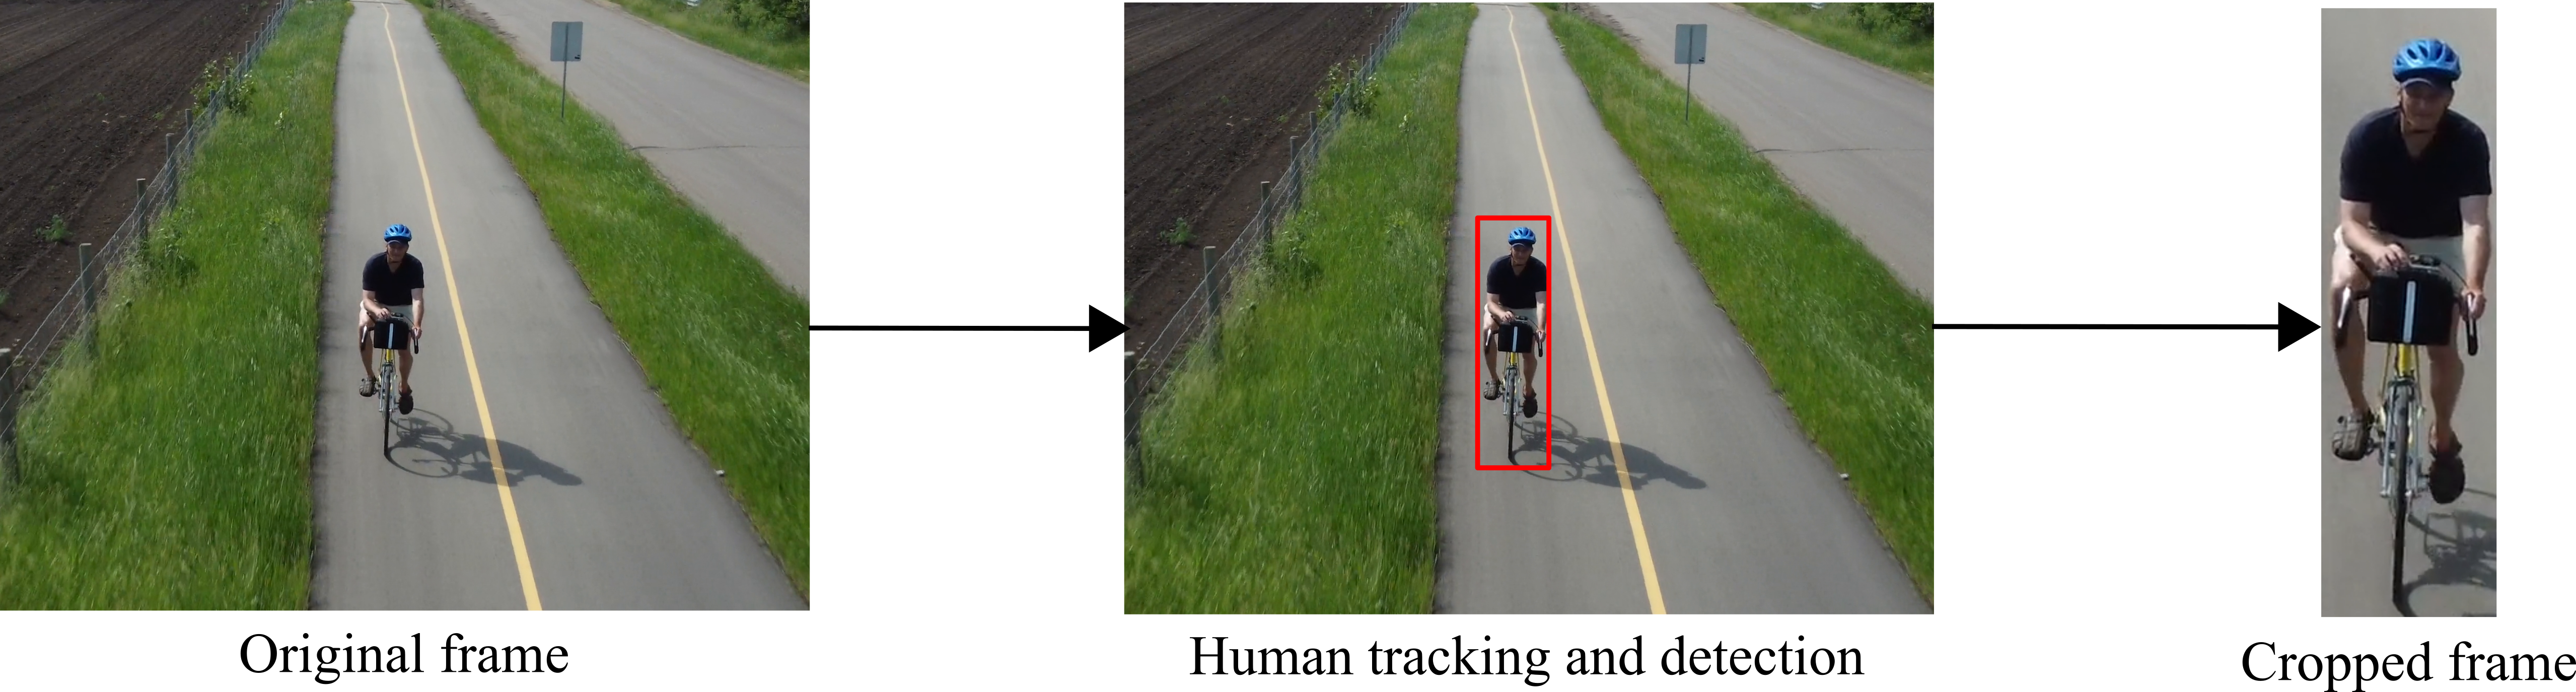
\includegraphics[width=1\textwidth]{Definitions/frame_cropped.png}
     \caption{Proposed human detection and tracking stage using FairMOT. \label{fig:human_detection_cropped}}     
\end{figure}

\subsection{Motion Features}
\label{sec:motion_features}
In the preceding section, the tracking process and the additional step of cropping each frame in the video to focus attention on a single individual and not on the entire scenario were described. The set of cropped frames will be referred to as the RGB data in the following sections. Once the cropped frames (RGB data) of the individuals have been obtained, as previously described, the next step is to preprocess them and calculate the motion features, which are composed of the optical flow and the pose features. The fusion of these features will be referred to as the motion data. 

The preprocessing phase aims to improve image classification by enhancing image features, such as the human pose. While some methods avoid feature engineering and rely on deep learning for automated inference, they can be computationally expensive. Different techniques, such as image resizing, noise reduction, and contrast enhancement, can be used to process each frame. This study generated two sets of frames using RGB and motion data. The set containing the RGB data, consisted of the cropped frames obtained in the previous section, are resized to 224$\times$224 pixels to match the input dimensions of the pretrained model used for feature extraction.

%RGB data is used to extract spatial features, while motion data is used to extract temporal information. 
%In this stage, preprocessing consists on resize the frames from The process involves bounding frames where the tracked subject is visible in the video, calculating optical flow, estimating 2D pose, and adjusting frame size. In the first step, described in \ref{sec:tracking}, the video frames are cropped using the bounding box coordinates generated by the FairMOT algorithm.% and resized to $224\times224$ pixels. 
%The cropped frames are used to create a new video clip, RGB clip, containing the RGB data. 

\begin{figure}[!ht]
     \centering
     \includegraphics[width=1\textwidth]{Definitions/preprocess.png}
     \caption{Proposed preprocessing stage. \label{fig:preprocessing}}     
\end{figure}


%For the second video clip, optical flow and pose estimation were computed from $RGBClip$ as shown in Figure \ref{fig:preprocessing}. For optical flow computation the Farneback method \cite{farneback} was used, while the 2D pose was estimated through the utilization of the mmpose framework \cite{mmpose2020}. Finally, the optical flow and the 2D pose data were combined to generate a new image containing both optical flow and the 2D pose for each video frame. Each new image are resized to $224\times224$ pixels, and a new video clip called $OpFlowPoseClip$ is generated with the new images.

For the motion data, optical flow and pose estimation were computed from the RGB data obtained in the previous section. 
%Figure \ref{fig:preprocessing} shows the output of this stage. 
In order to compute the optical flow, we used the Farneback method \cite{farneback}, while the mmpose framework \cite{mmpose2020} was used to estimate the 2D pose. The resulting data was then combined to create a new image containing optical flow and 2D pose for each video frame as it is shown in Figure \ref{fig:preprocessing}. Finally, each frame on the set of the RGB and motion data is resized to $224 \times 224$ pixels.

%by computing optical flow from $RGBClip_{n}$ using the Farneback method \cite{farneback}. 
%The 2D pose in Figure \ref{fig:pose_estimation_ex} is then estimated through the utilization of the mmpose framework \cite{mmpose2020}. 
%Then, the optical flow and the 2D pose data are combined to generate a new image, as shown in Figure \ref{fig:optical_flow_pose_ex} for each video frame. This process creates a new clip called $OpFlowPoseClip_{n}$. Finally, the frames of the newly added $RGBClip_{n}$ and $OpFlowPoseClip_{n}$ clips are resized to 224x224 pixels.

\subsection{Feature Extraction}
\label{sub:feature}
\begin{figure}[!ht]
     \centering
     \includegraphics[width=1\textwidth]{Definitions/feature_extraction.png}
     \caption{Feature extraction stage. \label{fig:feature_extraction}}     
\end{figure}
The next stage involves acquiring spatial and temporal features for the first 30 frames from the video. We use a transfer learning approach to leverage a robust model trained with images for this task. That allows us to extract spatial features from each video frame without the need to train a new model from scratch. The ConvNeXt-L model proposed in \cite{liu2022convnet} is used for this task. The feature extractor produces feature vectors of size 1536 for each frame. This output stage generates an array of 30 $\times$ 1536 features for each video, as 30 frames are used per video. This process generates two feature arrays per video: one with RGB features extracted from the RGB data and the other with extracted optical flow and pose features. 
Finally, we merged the features from RGB and motion data using concatenation as a fusion method. The feature arrays are concatenated per frame to create a single feature array of 30 $\times$ 3072 features. This approach utilizes the spatial features of the RGB data and the temporal features of the motion data as a single input for the classification model. 

\subsection{Training and Inference}
\label{sec:proposed_method}

The next steps involve the training and action inference after obtaining the feature vectors. The classification model, as shown in Figure \ref{fig:proposed_method}, consists of three main blocks that process spatial and temporal clues for classification and inference. 

\begin{figure}[!ht]
     \centering
     \includegraphics[width=1\textwidth]{Definitions/proposed_method.png}
     \caption{Classification model. \label{fig:proposed_method}}     
\end{figure}

After the feature fusion described in the subsection \ref{sub:feature}, batch normalization is applied to the data as a regularization step to avoid overfitting during training. The data is passed to the classification model shown in Figure \ref{fig:proposed_method}. The model implements a two-branch approach that processes the temporal features from the spatial data obtained with the pretrained model. 

In reference to the work developed by \cite{bai2018empirical}, Temporal Convolutional Networks (TCN) offer advantages over recurrent networks, such as a larger history compared to Long-Short Temporal Networks (LSTM). To take advantage of these features, the first stream of the proposed model includes TCN layers to exploit the temporal features between frames. The first stream of the model consists of two TCN layers with 64 and 128 filters, and dilatation factors of 1, 2, 4, 8, 16, and 32, followed by a max pooling of 3. Then, batch normalization is applied, followed by a TCN and a max pooling layer.

The second branch comprises two LSTM layers with 256 and 128 filters, respectively, each followed by a CNN and max pooling layer with 64 and 128 filters. It concludes with an LSTM layer with 64 filters. While TCNs are effective for storing large amounts of data, they do have some drawbacks when they are used for tasks with small amounts of memory. In the second stream of the model, we utilized LSTM layers to fully leverage the temporal features of the data. The outputs are then multiplied and passed to the fully connected stack, which consists of five layers: batch normalization, dropout, linear transformation, and two MLP layers.

\subsection{Data}
\label{subsec:data}

The development of HAR models presents certain challenges, particularly in relation to the data and the considerable computational resources required for training. In this study, we employed a bespoke dataset to develop the proposed HAR method, given that our computational resources were constrained by limited memory and graphical processing units. Accordingly, the custom dataset comprises five action classes: walking, running, cycling, and falling. This section provides a detailed description of the dataset above.

The process of obtaining the dataset was divided into two stages: data collection and selection. The initial stage entailed searching for videos containing the selected actions on the public datasets NTU RGB+D \cite{8713892}, UIUC \cite{10100742}, Weizmann \cite{ActionsAsSpaceTimeShapes_iccv05}, KTH \cite{1334462}, HMDB51 \cite{6126543}, HACS \cite{zhao2019hacs}, and UCF Sports \cite{soomro2012ucf101}. The graph in the Figure \ref{fig3} depicts the distribution of videos comprising the dataset assembled with these sources. 

\begin{figure}[ht]
\centering
   % 	     \begin{subfigure}[b]{0.65\textwidth}
%\includegraphics[width=\textwidth]{Definitions/data_distrib_pie.png}
      %  \end{subfigure}
   %\quad
    %\quad \quad  \quad \quad  \quad  \quad
 %       \begin{subfigure}[b]{0.4\textwidth}
    	
\includegraphics[width=0.65\textwidth]{Definitions/data_distrib_pie_sources.png}
  %      \end{subfigure} 
        %\quad
        %\begin{subfigure}[b]{0.36\textwidth}
    	
    	%\includegraphics[scale=0.5]{compuertas_3.PNG}
        %\end{subfigure}
        \caption{The distribution of the videos in the dataset according to the source from which they were extracted.} \label{fig3}
        \end{figure}

The characteristics of the videos extracted from each source are presented herein to gain insight into the nature of the videos utilized for training the proposed model. The datasets NTU RGB+D \cite{8713892} and UIUC \cite{10100742} comprise videos captured under controlled conditions. The videos depict a single individual performing a variety of actions. The camera remains fixed, the background remains static, and other persons are absent from the frames. Similarly, the Weizmann \cite{ActionsAsSpaceTimeShapes_iccv05} and KTH \cite{1334462} datasets contain videos captured under controlled conditions, though they are presented in grayscale.

\begin{figure}[ht!]
\includegraphics[width=13.7cm]{Definitions/data3.png}
\caption{The sample videos obtained from the Pexels, NTU RGB+D and MixKit websites.} \label{fig:samples}
\end{figure}

In contrast, the HMDB51 \cite{6126543}, HACS \cite{zhao2019hacs}, and UCF Sports \cite{soomro2012ucf101} datasets contain realistic videos with dynamic backgrounds. In certain instances, the entirety of the body is not visible. Furthermore, occlusions were extracted from motion pictures or television recordings. Moreover, in order to enhance the realism of the scenarios, additional data was sourced from the websites of Pexels \cite{pexels} and MixKit \cite{mixkitMixkitAwesome}. Figure \ref{fig:samples} presents several examples of the types of videos collected from the Pexels and MixKit websites. It also includes an illustration of a scenario involving controlled NTU RGB-D conditions.
\begin{figure}[ht]
\centering

\includegraphics[width=16cm]{Definitions/dist_vid_class.png}

\caption{The distribution of the videos is presented according to the class of membership and source of origin.} \label{fig4}
\end{figure}


As the proposed method depends upon extracting information from the poses, ensuring that the subjects are accurately identified and tracked throughout the video is of the utmost importance. To this end, the data selection process entailed verifying that the subjects on the video were detected and tracked for a minimum of seven frames and ensuring that the pose estimation could be executed successfully in each frame. Finally, 2,813 videos were collected. The videos were then divided into five subsets, comprising 189, 390, 490, 854, and 890 videos, respectively, and labeled according to the following categories: cycling, running, walking, drinking, and falling such as it is illustrated in the Figure \ref{fig4}. Due to the limited memory resources, the model was tested only on these videos. The data was divided into three subsets: 60\% for training, 30\% for validation, and 10\% for testing.

%\begin{figure}[ht!]
%\includegraphics[width=0.5\textwidth]{Definitions/data_distrib_pie_sources.png}
%\caption{Dataset samples.} \label{fig2}
%\end{figure}
%\begin{figure}[ht!]
%\includegraphics[width=0.7\textwidth]{Definitions/data_distrib_pie.png}
%\caption{Dataset samples.} \label{fig3}
%\end{figure}



%The dataset contains 2,813 videos divided into 189, 390, 490, 854, and 890 for cycling, running, walking, drinking, and falling class labels. The model was tested only with these videos due to limited memory resources. The data was split into three sets: 60\% for training, 30\% for validation, and 10\% for testing. 
%%%%%%%%%%%%%%%%%%%%%%%%%%%%%%%%%%%%%%%%%%
\section{Results}

In this section we present the results obtained from the experimental setup including the comparison of pretrained models and the performance of the presented method using different classes. For this reason, the section is organized as follows: the first part describes the dataset used and the implementation details, and the second part shows the experimental results.

\subsection{Experimental setup}
\textbf{Evaluation Dataset} The experiments were conducted on a custom dataset comprising five class labels. The dataset consisted of videos from public datasets, including NTU+RGBD-60, HMDB51, and KTH, which contained the actions of walking, running, cycling, drinking, or falling. Some videos were downloaded from pexels \cite{pexels} to create more variation in the dataset. %The dataset contains 2,813 videos divided into 189, 390, 490, 854, and 890 for cycling, running, walking, drinking, and falling class labels. 
The dataset has a standard three-split protocol, including training, test, and validation splits. In the end, 1,687 videos were used for training, 844 for testing, and 282 for validation.

\textbf{Implementation Details} %RGB, optical flow, and pose features were utilized for the experiments. 
For purposes of experimentation, RGB videos were employed for the extraction of RGB and motion features. Feature extraction was performed using a two-stream approach with fine-tuned pretrained models from the ImageNet dataset. In the first RGB stream, the input frames only contain the bounding box area with the detected object, while almost all the background of the image is ignored. The second stream's input is a frame that combines optical flow with pose. The optical flow was calculated using the Gunnar Farneback method, while the MMPose framework was used for 2D pose estimation. The frames were all 224 $\times$ 224 pixels in size.  We analyzed several pretrained models for feature extraction, including Inception-v3, MobileNet-v2, MobileNet-v3-L, VGG-16, VGG-19, Xception, and ConvNeXt-L. Each model generated feature vectors with varying numbers of features, ranging from 512 to 2048. The same feature extractor was used in both streams during the experiments. %The model inputs consisted of a minimum of 7 frames and a maximum of 30 frames. 
We trained the model using an SGD optimizer with an initial learning rate 1e-2 on a single GPU for all experiments. We implemented the model using TensorFlow and Keras frameworks.



\subsection{Experimental results}
\label{sec:results}

In this work, three experimental phases have been developed. In the first phase, there is a performance comparison between different pretrained models for feature extraction in the method proposed in Section \ref{sec:proposed_method}. The second experimental phase consisted of developing experiments with pretrained models using frozen weights, while the subsequent phase consisted of fine-tuning all the model parameters. For this purpose, the results obtained in each experimental stage are presented in this section.

\begin{table}[ht!]
\centering
\caption{Training results for four classes using pretrained models with frozen weights.\label{tab:comparison_pretrained}}
\begin{tabular}{@{}ccc@{}}
\toprule
\textbf{Model}          & \textbf{Train Acc. (\%)}  & \textbf{Validation Acc. (\%)}     \\ \midrule
Inception-v3   & 99                 & 90               \\
MobileNet-v2   & 96                 & 89               \\
MobileNet-v3-L & 100                & 92              \\
VGG-16         & 94                 & 86              \\
VGG-19         & 97                 & 91              \\
Xception       & 98                 & 89               \\
\textbf{ConvNeXt-L}     & 99        & \textbf{94}           \\ \bottomrule
\end{tabular}
\end{table}

The first experimental step was to replace the pretrained model used for feature extraction, shown in Figure \ref{fig:proposed_method}. For this purpose, Inception-v3, MobileNet-v2, MobileNet-v3-L, VGG16, VGG19, Xception, and ConvNeXt-L were selected. Additionally, it is worth noting that training was done using only four class labels; Table \ref{tab:comparison_pretrained} shows the training and testing results. The table shows that the ConvNeXt-L model provided the best results, followed by MobileNet-v3-L, while VGG16, the lightest model, obtained the worst result.


\begin{table}[ht!]
\centering
\caption{Performance comparison using pretrained model with frozen weights and fine tuning with the RGB data. \label{tab:rgb_frozen_vs_fn}}
\begin{tabular}{c|cc|cc}
       \textbf{RGB}  & \multicolumn{2}{c|}{\textbf{Frozen weights}} & \multicolumn{2}{c}{\textbf{Fine tuning}} \\ \hline
\textbf{No. classes} & \textbf{Train (\%)}        & \textbf{Test (\%)}        & \textbf{Train (\%)}       & \textbf{Test (\%)}      \\ \hline
3                    & 95                    & 86                   & 97.98                & 90.65              \\
4                    & 99                    & 90                   & 97.62                & 93.71              \\
5                    & 66                    & 63                   & 96.23                & 90.93              \\ \hline
Avg.                 & 86.67                 & 79.67               &  97.28               &  91.66
\end{tabular}
\end{table}

The ConvNeXt-L model was selected for the following experiments based on previous results. These experiments show the performance of the model using original weights during training and when full fine-tuning is performed. Only RGB data were used for preliminary experiments to feed the proposed model. Table \ref{tab:rgb_frozen_vs_fn} shows the results obtained when three, four, and five class labels were used during training. Experiments demonstrated that implementing fine-tuning improves performance accuracy of the proposal, increasing it by up to 12\%. Additionally, significant improvement was observed during training with five classes. Initial experiments showed accuracy barely surpassing 60\%, but with fine tuning, results increased to 90.93\% using only RGB data.

\begin{table}[ht!]
\centering
\caption{Performance comparison using pretrained model with frozen weights and fine tuning with the fusion of RGB and motion features. \label{tab:motion_frozen_vs_fn}}
\begin{tabular}{c|cc|cc}
\textbf{RGB + Motion}& \multicolumn{2}{c|}{\textbf{Frozen weigths}} & \multicolumn{2}{c}{\textbf{Fine tuning}} \\ \hline
\textbf{No. classes} & \textbf{Train (\%)}        & \textbf{Test (\%)}        & \textbf{Train (\%)}       & \textbf{Test (\%)}      \\ \hline
3                    &  95                   & 86                   &  95.95               &  90.03             \\
4                    &  99                   & 94                   &  98.98               &  94.90             \\
5                    &  76                   & 73                   &  94.46               &  92.11             \\ \hline
Avg.                 &  90                 & 84.3               &  96.46               &  92.35
\end{tabular}
\end{table}

One of the goals of this proposal is to use motion information to enrich temporal data and take advantage of appearance and movement information. In the next experimental stage, features from the RGB and Motion data were fused. Results similar to the previous stage were presented in Table \ref{tab:motion_frozen_vs_fn}, showing the training results when frozen weights were used and when fine-tuning was done. Similar to the previous results, the fine-tuning test results show an average of 91.66\% and 92.35\% in Tables \ref{tab:rgb_frozen_vs_fn} and \ref{tab:motion_frozen_vs_fn}, respectively. 

% Please add the following required packages to your document preamble:
% \usepackage{booktabs}
%\begin{table}[]
%\begin{tabular}{@{}cccclcl@{}}
%\toprule
%Model          & Train Acc. & Test Acc. & Validation Acc. & Pretrained params & Params    & Total params \\ \midrule
%Inception-v3   & 99         & 91        & 90              & 21,802,784        & 6,634,524 & 28,437,308   \\
%MobileNet-v2   & 96         & 90        & 89              & 2,257,984         & 4,668,444 & 2,724,828    \\
%MobileNet-v3-L & 100        & 93        & 92              & 2,996,352         & 3,849,244 & 6,845,596    \\
%VGG-16         & 94         & 89        & 86              & 14,714,688        & 2,702,364 & 17,417,052   \\
%VGG-19         & 97         & 92        & 91              & 20,024,384        & 2,702,364 & 22,726,748   \\
%Xception       & 98         & 89        & 89              & 20,861,480        & 6,634,524 & 27,496,004   \\
%ConvNeXt-L     & 99         & 94        & 94              & 196,230,336       & 5,323,804 & 201,554,140  \\ \bottomrule
%\end{tabular}
%\end{table}
%%%%%%%%%%%%%%%%%%%%%%%%%%%%%%%%%%%%%%%%%%
\section{Discussion}

This work presents a method for performing HAR in videos using a transfer learning approach for feature extraction. Two different transfer learning schemes were adopted. The first scheme involved using the original weights of the models to evaluate the performance of the seven models on the proposal shown in Figure \ref{fig:proposed_method}. The second scheme involved retraining all weights of the models to improve the resulting accuracy of the proposal. 

Regarding the results presented in Tables \ref{tab:comparison_pretrained}, \ref{tab:rgb_frozen_vs_fn}, and \ref{tab:motion_frozen_vs_fn} of Section \ref{sec:results}, it is encouraging to note that using the original weights of the models leads to accuracies ranging from 86\% to 94\%, with the ConvNeXt-L model performing the best. As a result, the next set of reported experiments used the ConvNeXt-L model. As part of preliminary experiments, we studied the behavior of the model when using only the RGB data generated in Section \ref{sec:motion_features}. Under this scheme, the model achieved 90\% accuracy when trained with four class labels, compared to the 63\% accuracy obtained when five class labels were included.

To improve the performance of the proposed model, the next set of experiments involved feeding the model with the RGb and motion data. The use of motion features was expected to enhance the model's performance. As expected, the results, shown in Table \ref{tab:motion_frozen_vs_fn}, improved up to 10\%. The best improvement was observed during the training of five classes, achieving a 73\% accuracy while when four classes were trained, the accuracy achieved 94\%, an improvement of four percentage points. These results prove that motion features enhance the model's performance.

The weights of the pretrained models were retrained to increase the accuracy of the proposed model. Training under this scheme and using the RGB data resulted in an improved accuracy from 3.71\% to 27.93\%. This gave us an average accuracy of 91.8\% when training with three, four, and five classes, a considerable improvement compared to the 79.7\% achieved when training with the original weights. The results of using both RGB and Motion data were observed to be interesting, as the resulting accuracy average of 92.4\% was similar to the case with only RGB data while presenting an improvement of 0.9\% to 19.11\%. The training was conducted with five class labels, which yielded the best results.

%%%%%%%%%%%%%%%%%%%%%%%%%%%%%%%%%%%%%%%%%%
\section{Conclusions an Future Work}
In this work a method for HAR that utilizes CNN, LSTM, and transfer learning is presented. The workflow involves human detection and tracking, video preprocessing, feature extraction, and action inference. The conclusions derived from this work and possible future directions for work are presented next. 

\subsection{Conclusions}
%The proposed method focuses on the subject performing the actions by using the bounding box of the detected subject. This results in a tracking-based model that takes advantage of spatial and temporal features. Seven pretrained models were examinated for feature extraction, and the ConvNeXt model demonstrating the most promising performance, as illustrated in Table \ref{tab:comparison_pretrained}; however, a lightweight model could be chosen to save time and resources, even at the cost of accuracy. Due to limited resources, specifically in terms of memory, the work was restricted to five action classes: cycling, walking, running, drinking, and falling. This resulted in a dataset with 2,813 videos encompassing a diverse range of scenarios, including both controlled (67.1\%) and uncontrolled scenes (32.9\%). 

%Conversely, although some researchers propose the use of two-stream models with a dedicated stream for spatial and temporal information, in this work, the presented model employs a pretrained model for spatial feature extraction, which feeds a two-stream network for the processing of temporal data with LSTM and TCN layers. Finally, the outputs of the two streams are combined into a single feature vector for the input video. The resulting model exhibited test accuracy of 90.3\%, 94.9\%, and 92.11\% with three, four, and five classes, respectively. Upon examination of the model's performance with the imbalanced dataset, it was observed that during training, the results did not exhibit a clear bias towards any specific class. This was evident in the precision score of around 92.4\%, which was calculated by averaging the performance of the model across three, four, and five classes shown in Table \ref{tab:motion_frozen_vs_fn}.

This paper presents a tracking-based method for the HAR task. The goal of the method is to identify the human movement patterns associated with the execution of these action classes. To achieve this goal, a multiple object tracker, namely FairMOT, was employed to track the humans within the video sequences. Subsequently, the bounding boxes identified by FairMOT were employed to crop the video frames around the detected humans and then, motion data were estimated through the implementation of an optical flow and pose estimation algorithms. 

Afterwards, feature extraction is conducted. Using a pretrained model the method exploit the spatial information on the RGB data while temporal features were extracted using a motion data. Seven pretrained models were examinated for feature extraction, and the ConvNeXt-L model demonstrating the most promising performance, as illustrated in Table \ref{tab:comparison_pretrained}; however, a lightweight model could be chosen to save time and resources, even at the cost of accuracy.
The resulting features from the ConvNeXt-L model were introduced to a two-stream model. While some researchers propose the use of two-stream models with a dedicated stream for spatial and temporal information, in this work, the presented model employs a pretrained model for spatial feature extraction, which feeds a two-stream network for the processing of temporal data with LSTM and TCN layers. The outputs of the two streams are then combined into a single feature vector for the input video. 

The resulting model exhibited test accuracy of 90.3\%, 94.9\%, and 92.11\% with three, four, and five classes, respectively improving the results when only RGB data is employed. It was observed that the model exhibited higher accuracy results when trained with four classes. This indicates that the patterns identified by the model during training allow for more effective differentiation between the four classes used during training. However, further investigation is necessary to confirm these findings. In particular, future work should consider training the model with a wider range of classes.

Upon examination of the model's performance with the imbalanced dataset, it was observed that during training, the results did not exhibit a clear bias towards any specific class. 
The model exhibited precision of approximately 92.35\%, which was calculated by averaging its performance across three, four, and five classes, as detailed in Table \ref{tab:motion_frozen_vs_fn}. 
%This was seen in the precision score of around 92.35\%, which was calculated by averaging the performance of the model across three, four, and five classes shown in Table \ref{tab:motion_frozen_vs_fn}. 
Due to limited resources, specifically in terms of memory, the work was restricted to five action classes: cycling, walking, running, drinking, and falling. This resulted in a dataset with 2,813 videos encompassing a diverse range of scenarios, including both controlled (67.1\%) and uncontrolled scenes (32.9\%). Although the dataset encompasses a diverse range of scenarios, including both controlled and uncontrolled conditions, the experimental stage could be enhanced for future studies. This could be achieved by increasing the variety of the dataset with respect to uncontrolled scenarios. This would enable the observation of whether the performance of the model is maintained or enhanced.

\subsection{Future Work}
Based on the work presented in this paper, we have identified some essential points for future development. One crucial aspect for real-world applications is increasing the number of classes the model recognizes. Currently, there are datasets containing up to 700 class labels. However, a significant amount of computational resources is required for training, but with pretrained models as ConvNeXt-L could be help develop deeper models or ensembling different classifiers to achieve the task. Additionally, action recognition serves as a good starting point for automatic human behavior understanding. Therefore, developing models for complex action recognition, action tracking, and even multilabel recognition is essential. Finally, transformers have been gaining attention in computer vision. It would be useful to develop a study to compare transfer learning approaches using transformers and video pretrained models, rather than only using convolutional approaches. 

%%%%%%%%%%%%%%%%%%%%%%%%%%%%%%%%%%%%%%%%%%
%\section{Patents}

%This section is not mandatory, but may be added if there are patents resulting from the work reported in this manuscript.

%%%%%%%%%%%%%%%%%%%%%%%%%%%%%%%%%%%%%%%%%%
%\vspace{6pt} 

%%%%%%%%%%%%%%%%%%%%%%%%%%%%%%%%%%%%%%%%%%
%% optional
%\supplementary{The following supporting information can be downloaded at:  \linksupplementary{s1}, Figure S1: title; Table S1: title; Video S1: title.}

% Only for journal Methods and Protocols:
% If you wish to submit a video article, please do so with any other supplementary material.
% \supplementary{The following supporting information can be downloaded at: \linksupplementary{s1}, Figure S1: title; Table S1: title; Video S1: title. A supporting video article is available at doi: link.}

% Only for journal Hardware:
% If you wish to submit a video article, please do so with any other supplementary material.
% \supplementary{The following supporting information can be downloaded at: \linksupplementary{s1}, Figure S1: title; Table S1: title; Video S1: title.\vspace{6pt}\\
%\begin{tabularx}{\textwidth}{lll}
%\toprule
%\textbf{Name} & \textbf{Type} & \textbf{Description} \\
%\midrule
%S1 & Python script (.py) & Script of python source code used in XX \\
%S2 & Text (.txt) & Script of modelling code used to make Figure X \\
%S3 & Text (.txt) & Raw data from experiment X \\
%S4 & Video (.mp4) & Video demonstrating the hardware in use \\
%... & ... & ... \\
%\bottomrule
%\end{tabularx}
%}

%%%%%%%%%%%%%%%%%%%%%%%%%%%%%%%%%%%%%%%%%%
\authorcontributions{ ``Conceptualization, E.L.-L.; methodology, E.L.-L. and H.S.; software, E.L.-L.; validation, E.L.-L., H.S. and E.R.-E.; formal analysis, E.L.-L; investigation, E.L.-L.; resources, E.R.-E. and H.S.; data curation, E.L.-L.; writing---original draft preparation, E.L.-L.; writing---review and editing, H.S. and E.R.-E..}

\funding{``This research received no external funding''}


\dataavailability{We encourage all authors of articles published in MDPI journals to share their research data. In this section, please provide details regarding where data supporting reported results can be found, including links to publicly archived datasets analyzed or generated during the study. Where no new data were created, or where data is unavailable due to privacy or ethical restrictions, a statement is still required. Suggested Data Availability Statements are available in section ``MDPI Research Data Policies'' at \url{https://www.mdpi.com/ethics}.} 

\acknowledgments{The authors would like to thank the Instituto Politécnico Nacional and Secretar\'ia de Investigaci\'on y Posgrado (SIP-IPN) under projects 20231622, 20232570, 20242742 and 20240956 for the economical support to undertake this research and the Comisión de Operación y Fomento de Actividades Académicas (COFAA-IPN). E. López thanks CONAHCYT for the scholarship granted to undertake her PhD studies.}

\conflictsofinterest{The authors declare no conflict of interest.} 

%%%%%%%%%%%%%%%%%%%%%%%%%%%%%%%%%%%%%%%%%%
%% Only for journal Encyclopedia
%\entrylink{The Link to this entry published on the encyclopedia platform.}

\abbreviations{Abbreviations}{
The following abbreviations are used in this manuscript:\\

\noindent 
\begin{tabular}{@{}ll}
HAR & Human Action Recognition\\
DL & Deep Learning\\
CNN & Convolutional Neural Network\\
TCN & Temporal Convolutional Network\\
SGD & Stochastic Gradient Descent \\
MOT & Multi-Object Tracking\\
VGG & Visual Geometry Group \\
LSTM & Long Short Term Memory \\
GPU & Graphics Processing Unit \\
HMDB & Human Motion Database \\
RGB & Red Green Blue \\
BN & Batch Normalization \\
GP & Global Pooling \\
MP & Max Pooling \\
MLP & Multi Layer Perceptron \\
\end{tabular}
}

%%%%%%%%%%%%%%%%%%%%%%%%%%%%%%%%%%%%%%%%%%
%% Optional
%\appendixtitles{no} % Leave argument "no" if all appendix headings stay EMPTY (then no dot is printed after "Appendix A"). If the appendix sections contain a heading then change the argument to "yes".
%\appendixstart
%\appendix
%\section[\appendixname~\thesection]{}
%\subsection[\appendixname~\thesubsection]{}
%The appendix is an optional section that can contain details and data supplemental to the main text---for example, explanations of experimental details that would disrupt the flow of the main text but nonetheless remain crucial to understanding and reproducing the research shown; figures of replicates for experiments of which representative data are shown in the main text can be added here if brief, or as Supplementary Data. Mathematical proofs of results not central to the paper can be added as an appendix.

%\begin{table}[H] 
%\caption{This is a table caption.\label{tab5}}
%\newcolumntype{C}{>{\centering\arraybackslash}X}
%\begin{tabularx}{\textwidth}{CCC}
%\toprule
%\textbf{Title 1}	& \textbf{Title 2}	& \textbf{Title 3}\\
%\midrule
%Entry 1		& Data			& Data\\
%Entry 2		& Data			& Data\\
%\bottomrule
%\end{tabularx}
%\end{table}

%\section[\appendixname~\thesection]{}
%All appendix sections must be cited in the main text. In the appendices, Figures, Tables, etc. should be labeled, starting with ``A''---e.g., Figure A1, Figure A2, etc.

%%%%%%%%%%%%%%%%%%%%%%%%%%%%%%%%%%%%%%%%%%
\begin{adjustwidth}{-\extralength}{0cm}
%\printendnotes[custom] % Un-comment to print a list of endnotes

\reftitle{References}

% Please provide either the correct journal abbreviation (e.g. according to the “List of Title Word Abbreviations” http://www.issn.org/services/online-services/access-to-the-ltwa/) or the full name of the journal.
% Citations and References in Supplementary files are permitted provided that they also appear in the reference list here. 

%=====================================
% References, variant A: external bibliography
%=====================================
%\bibliography{your_external_BibTeX_file}

%=====================================
% References, variant B: internal bibliography
%=====================================
%\begin{thebibliography}{999}
%\bibliographystyle{splncs04}
\bibliography{biblio}
%\end{thebibliography}

% If authors have biography, please use the format below
%\section*{Short Biography of Authors}
%\bio
%{\raisebox{-0.35cm}{\includegraphics[width=3.5cm,height=5.3cm,clip,keepaspectratio]{Definitions/author1.pdf}}}
%{\textbf{Firstname Lastname} Biography of first author}
%
%\bio
%{\raisebox{-0.35cm}{\includegraphics[width=3.5cm,height=5.3cm,clip,keepaspectratio]{Definitions/author2.jpg}}}
%{\textbf{Firstname Lastname} Biography of second author}

% For the MDPI journals use author-date citation, please follow the formatting guidelines on http://www.mdpi.com/authors/references
% To cite two works by the same author: \citeauthor{ref-journal-1a} (\citeyear{ref-journal-1a}, \citeyear{ref-journal-1b}). This produces: Whittaker (1967, 1975)
% To cite two works by the same author with specific pages: \citeauthor{ref-journal-3a} (\citeyear{ref-journal-3a}, p. 328; \citeyear{ref-journal-3b}, p.475). This produces: Wong (1999, p. 328; 2000, p. 475)

%%%%%%%%%%%%%%%%%%%%%%%%%%%%%%%%%%%%%%%%%%
%% for journal Sci
%\reviewreports{\\
%Reviewer 1 comments and authors’ response\\
%Reviewer 2 comments and authors’ response\\
%Reviewer 3 comments and authors’ response
%}
%%%%%%%%%%%%%%%%%%%%%%%%%%%%%%%%%%%%%%%%%%
\PublishersNote{}
\end{adjustwidth}
\end{document}

